% ============================================================
% ONERA M6 -- ICE ACCRETION
% ============================================================

\section[Ice]{\textbf{Ice Accretion}}

% ============================================================
% ONERA M6 -- Ice Mass Grid Convergence
% ============================================================

\begin{frame}{\small ONERA M6 -- Ice Mass Grid Convergence (15 Bins)}
\scriptsize

\begin{columns}[T,onlytextwidth]

\begin{column}{0.50\textwidth}
    \centering
    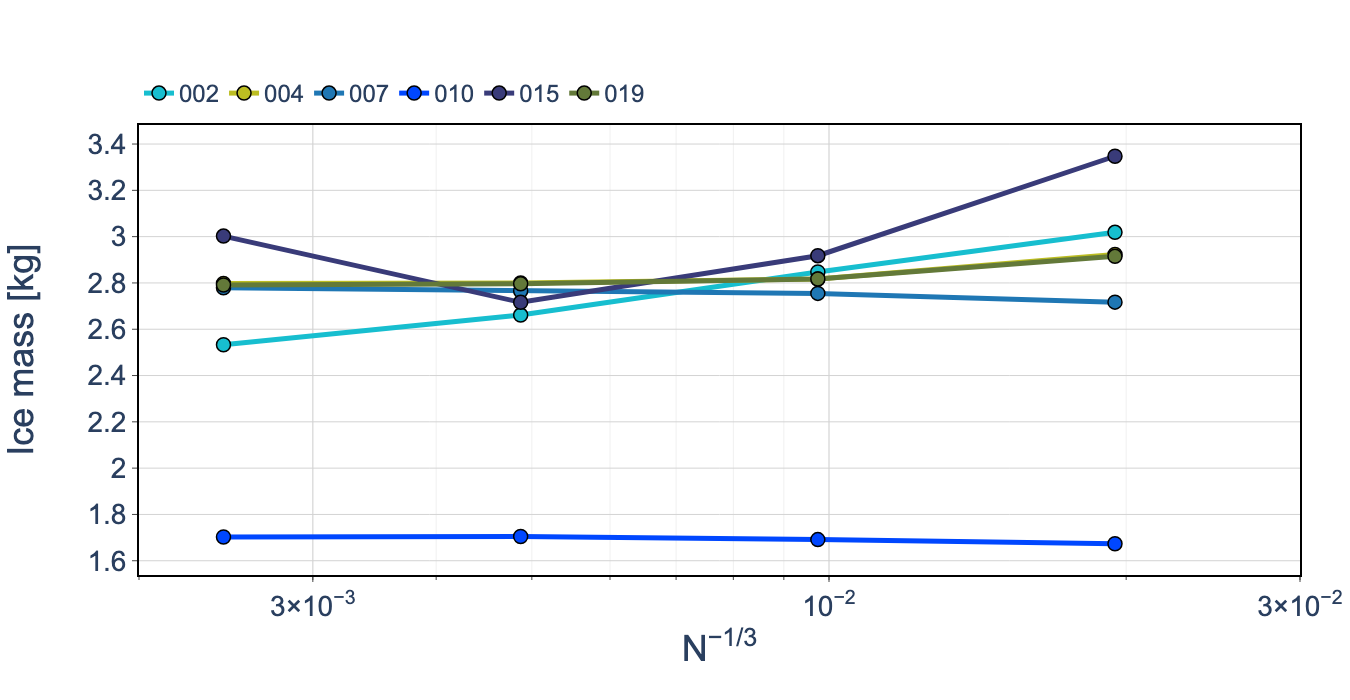
\includegraphics[width=0.94\textwidth]{FIGURES/ICE_ACCRETION/tc_oneram6_ice_mass_vs_n_1mm_bins15_all_grid_levels.png}

    \vspace{0.05cm}

    \textbf{Ice Mass}
\end{column}

\begin{column}{0.50\textwidth}
    \centering
    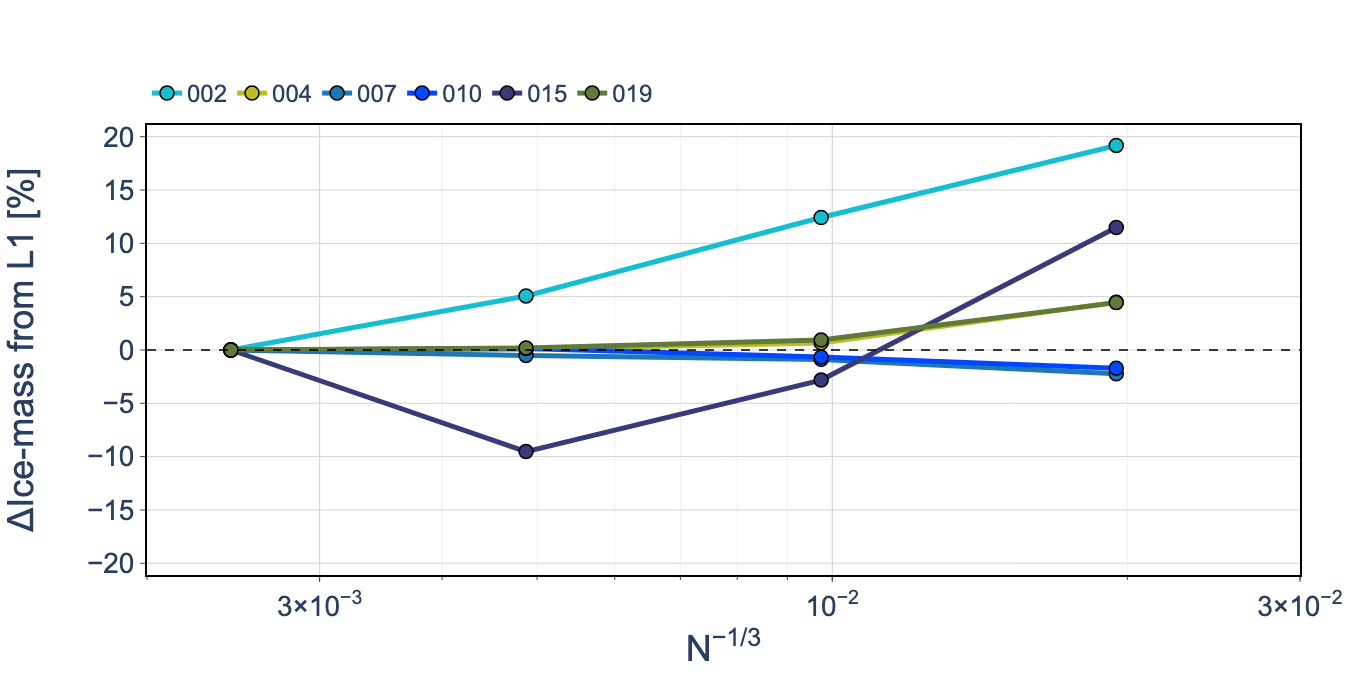
\includegraphics[width=0.94\textwidth]{FIGURES/ICE_ACCRETION/tc_oneram6_ice_mass_vs_n_1mm_bins15_all_grid_levels_relative_to_l1.png}

    \vspace{0.05cm}

    \textbf{Relative to L1}
\end{column}

\end{columns}

\vspace{0.05cm}

{\centering\textbf{Roughness: 1 mm}\par}

\vspace{0.10cm}

\begin{block}{\scriptsize Assessment}
\begin{itemize}
    \item Ice-mass grid sensitivity is strongly submission-dependent.
    \item Relative to L1, coarse-grid differences remain below approximately $5\%$ for several submissions, but reach approximately $20\%$ and $11\%$ for selected submissions on L4.
    \item Considerable code-to-code differences remain on L1 and are generally larger than the grid-refinement effect.
\end{itemize}
\end{block}

\end{frame}


% ============================================================
% ONERA M6 -- Ice Mass Droplet-Distribution Sensitivity
% ============================================================

\begin{frame}{\small ONERA M6 -- Ice Mass Sensitivity to Droplet Distribution}
\scriptsize

\begin{columns}[T,onlytextwidth]

\begin{column}{0.50\textwidth}
    \centering
    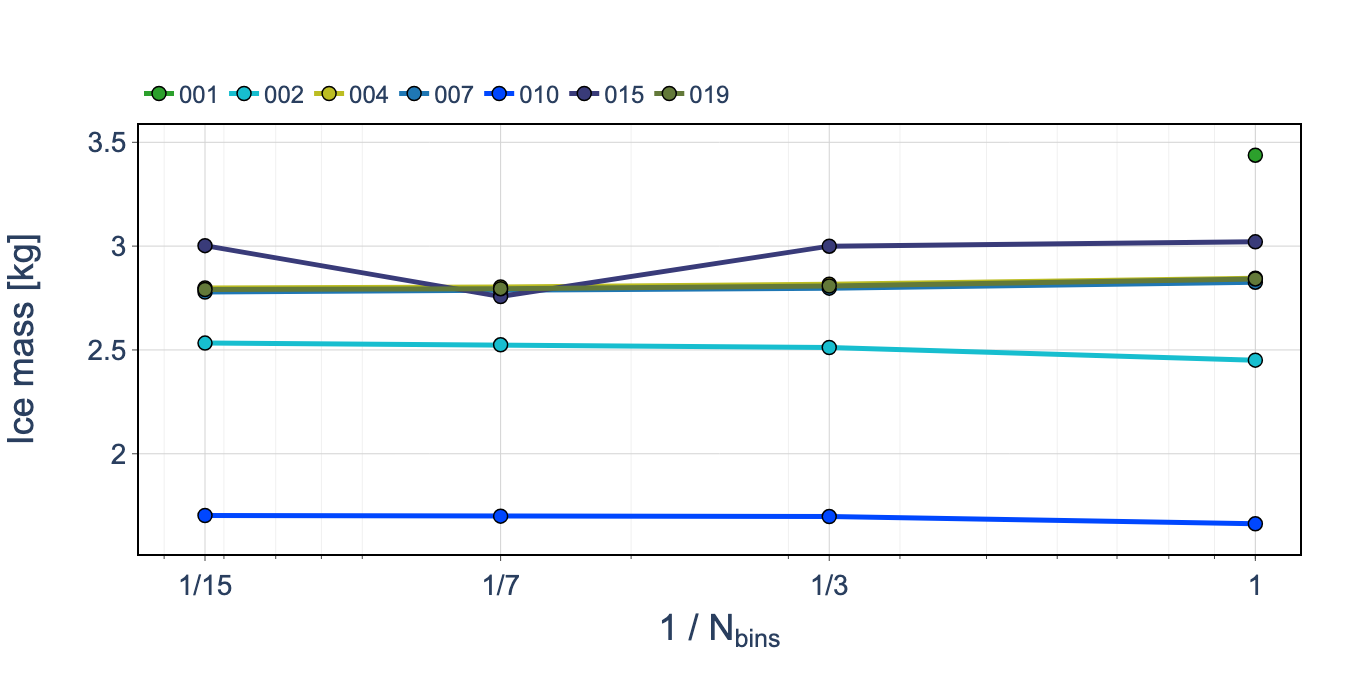
\includegraphics[width=0.94\textwidth]{FIGURES/ICE_ACCRETION/tc_oneram6_ice_mass_vs_n_1mm_l1_vs_inverse_bins.png}

    \vspace{0.05cm}

    \textbf{Ice Mass}
\end{column}

\begin{column}{0.50\textwidth}
    \centering
    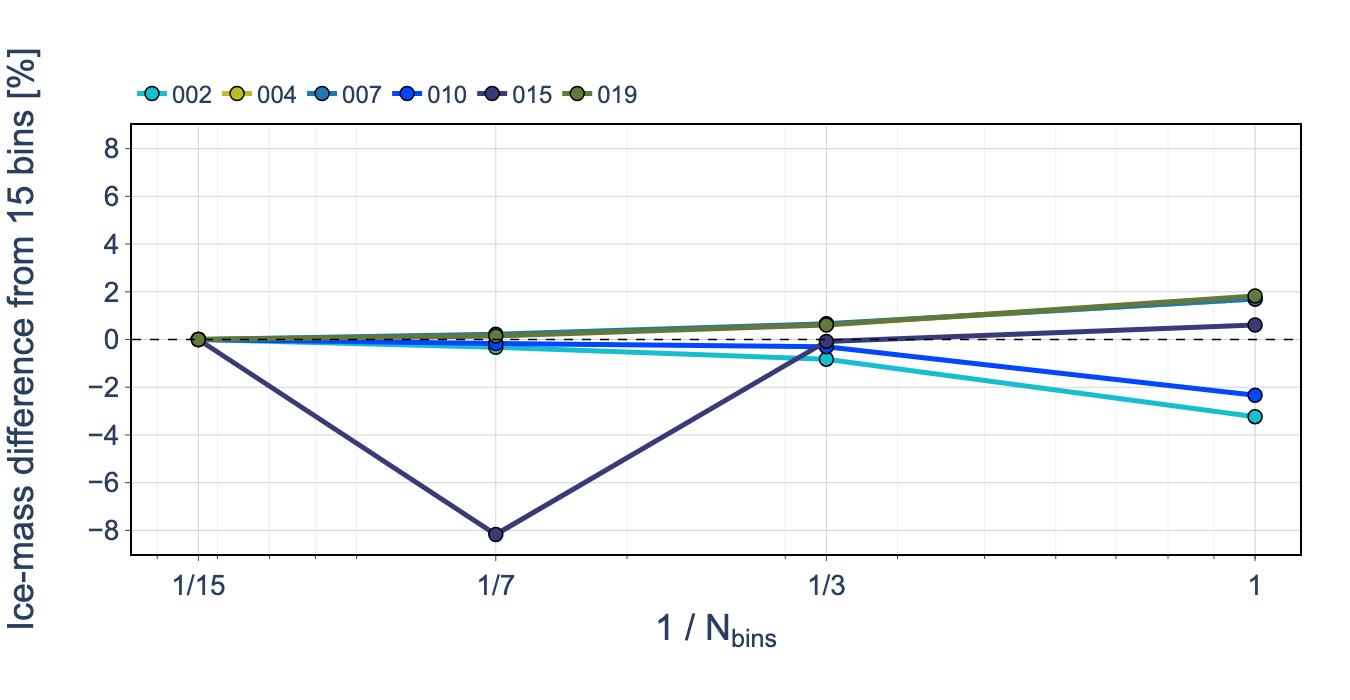
\includegraphics[width=0.94\textwidth]{FIGURES/ICE_ACCRETION/tc_oneram6_ice_mass_vs_n_1mm_l1_vs_inverse_bins_relative_to_bins15.png}

    \vspace{0.05cm}

    \textbf{Relative to 15 Bins}
\end{column}

\end{columns}

\vspace{0.05cm}

{\centering\textbf{L1 -- Roughness: 1 mm}\par}

\vspace{0.10cm}

\begin{block}{\scriptsize Assessment}
\begin{itemize}
    \item Ice mass exhibits limited sensitivity to droplet-distribution resolution for most submissions.
    \item Relative differences from the 15-bin prediction generally remain within approximately $3\%$, with one isolated 7-bin deviation of approximately $8\%$.
    \item Code-to-code differences remain considerably larger than the droplet-distribution effect.
    \item This behavior is consistent with the weak distribution sensitivity previously observed for the integrated impinged water mass.
\end{itemize}
\end{block}

\end{frame}


% ============================================================
% ONERA M6 -- Ice and Evaporation Mass Ratios
% ============================================================

\begin{frame}{\small ONERA M6 -- Ice and Evaporation Mass Ratios}
\scriptsize

\begin{columns}[T,onlytextwidth]

\begin{column}{0.50\textwidth}
    \centering
    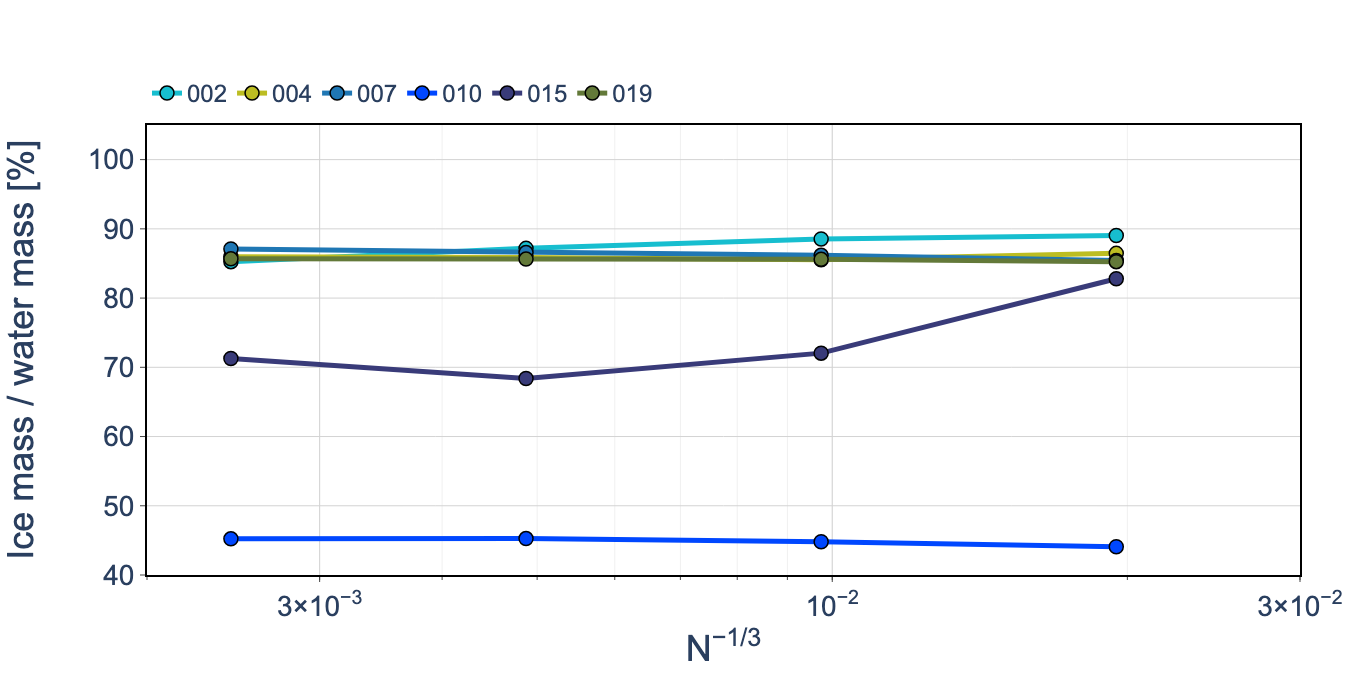
\includegraphics[width=\textwidth]{FIGURES/ICE_ACCRETION/tc_oneram6_ice_to_water_ratio_vs_n_required_bins15.png}

    \vspace{0.05cm}

    {\scriptsize\textbf{Ice / Water}}
\end{column}

\begin{column}{0.50\textwidth}
    \centering
    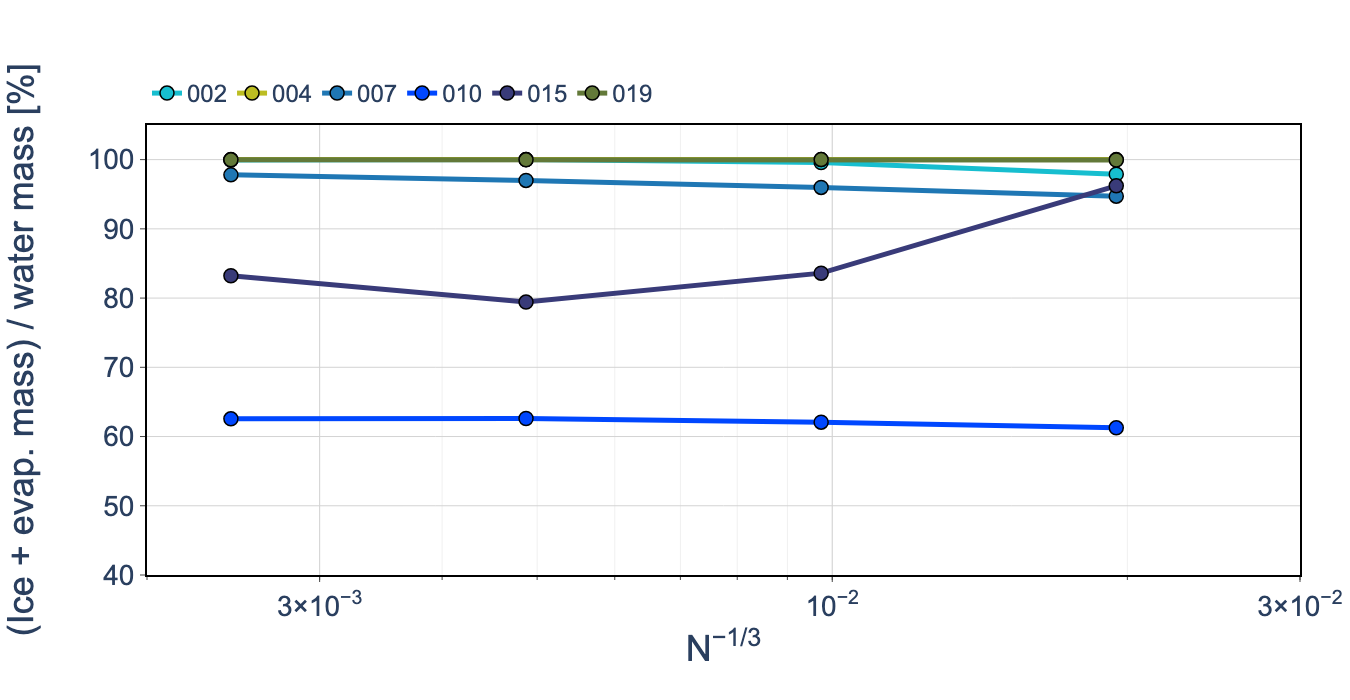
\includegraphics[width=\textwidth]{FIGURES/ICE_ACCRETION/tc_oneram6_ice_evap_to_water_ratio_vs_n_required_bins15.png}

    \vspace{0.05cm}

    {\scriptsize\textbf{(Ice + Evaporation) / Water}}
\end{column}

\end{columns}

\vspace{0.15cm}

\begin{block}{\scriptsize Assessment}
\begin{itemize}
    \item Most submissions convert approximately $85$--$89\%$ of the impinged water mass into ice.
    \item Accounting for evaporation brings the mass balance close to $100\%$ for several submissions, indicating that evaporation explains a significant fraction of the non-accreted water.
    \item Lower ratios for some submissions are consistent with reported water shedding, which provides an additional pathway for the impinged water mass.
\end{itemize}
\end{block}

\end{frame}


% ============================================================
% ONERA M6 -- Ice Mass Roughness Sensitivity
% ============================================================

\begin{frame}{\small ONERA M6 -- Ice Mass Roughness Sensitivity}
\scriptsize

\centering

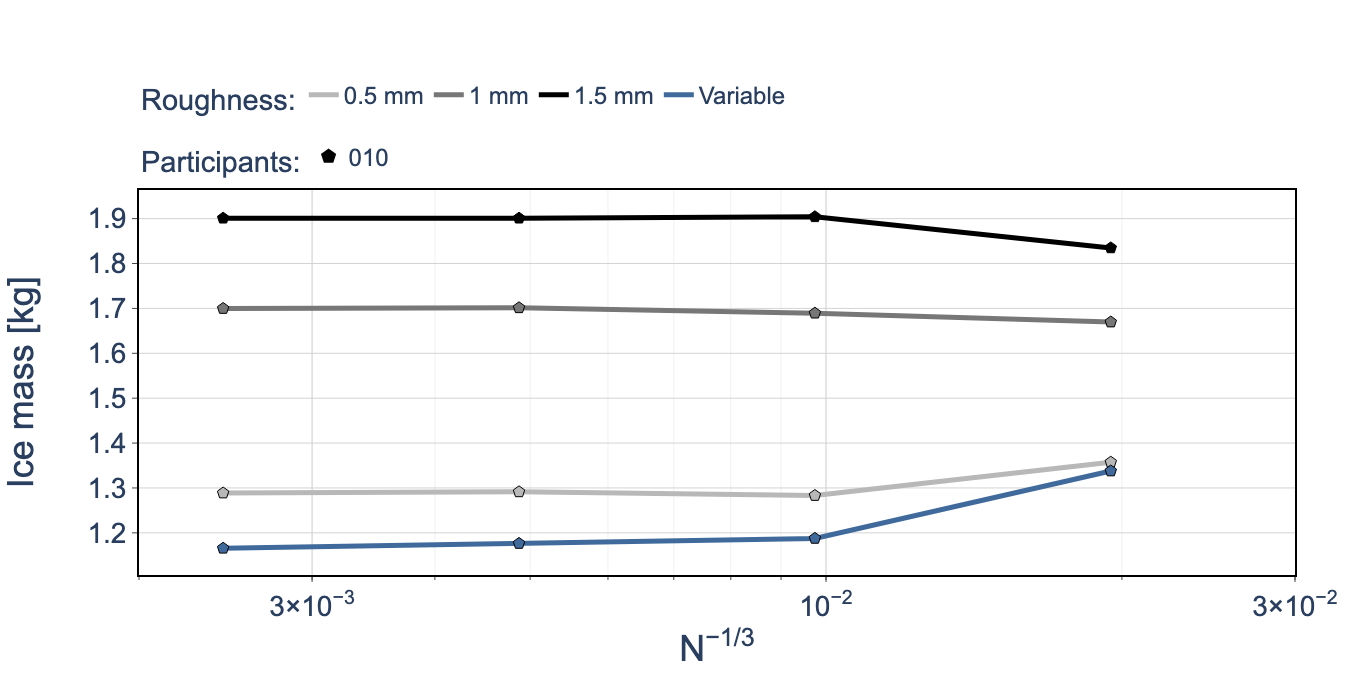
\includegraphics[width=0.70\textwidth]{FIGURES/ICE_ACCRETION/tc_oneram6_010_ice_mass_vs_n_bins07_grouped_roughness.png}

\vspace{0.10cm}

\begin{block}{\scriptsize Assessment}
\begin{itemize}
    \item One submission provided additional results for multiple prescribed roughness heights.
    \item Ice mass increases substantially with roughness, from approximately $1.3$ kg at $k_s=0.5$ mm to $1.9$ kg at $k_s=1.5$ mm on L1.
\end{itemize}
\end{block}

\end{frame}


% ============================================================
% ONERA M6 -- Ice Shapes
% ============================================================

\begin{frame}{\small ONERA M6 -- Ice Shapes (L1, 15 Bins)}
\scriptsize

% ------------------------------------------------------------
% Representative mid-span slice
% ------------------------------------------------------------
\only<1>{

\centering

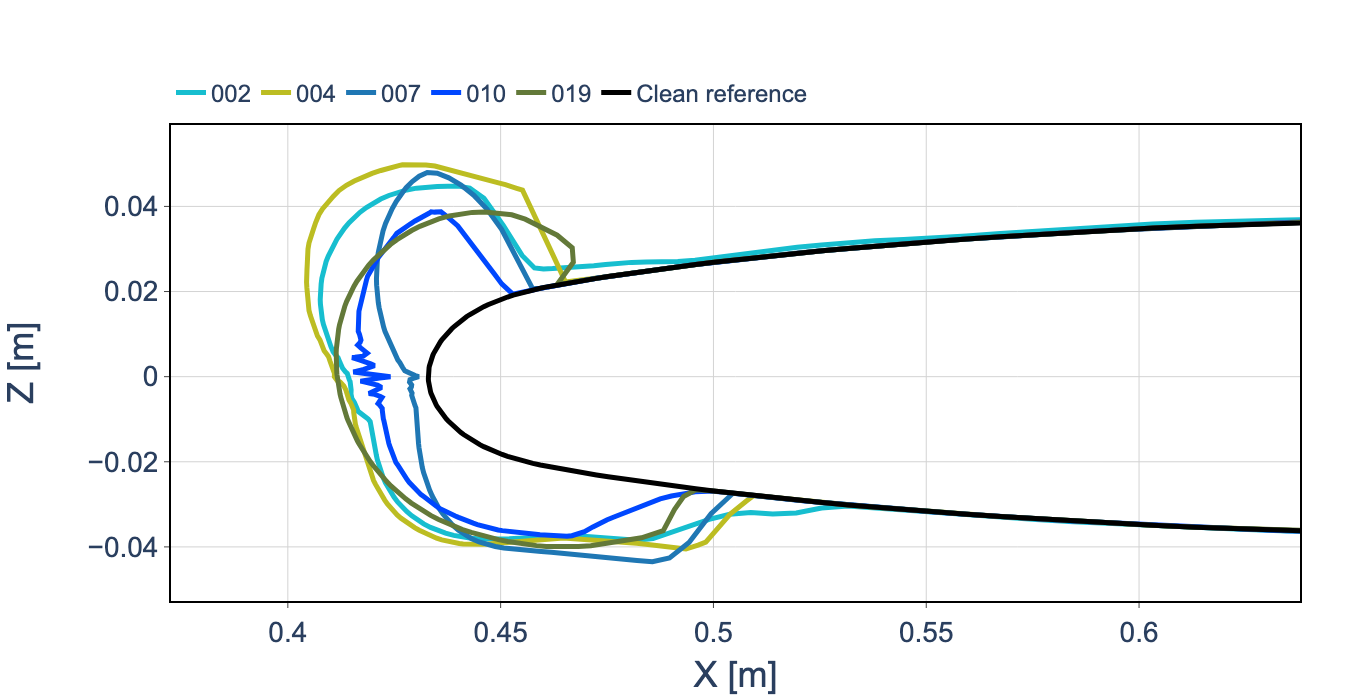
\includegraphics[width=0.6\textwidth]{FIGURES/ICE_SHAPES/tc_oneram6_L1_single_layer_ice_shape_slice_0p75_bins15_roughness_1mm.png}

\vspace{0.05cm}

{\scriptsize\textbf{$y=0.75$ m -- Roughness: 1 mm}}

}

% ------------------------------------------------------------
% Other spanwise slices
% ------------------------------------------------------------
\only<2>{

\begin{columns}[T,onlytextwidth]

\begin{column}{0.50\textwidth}
    \centering

    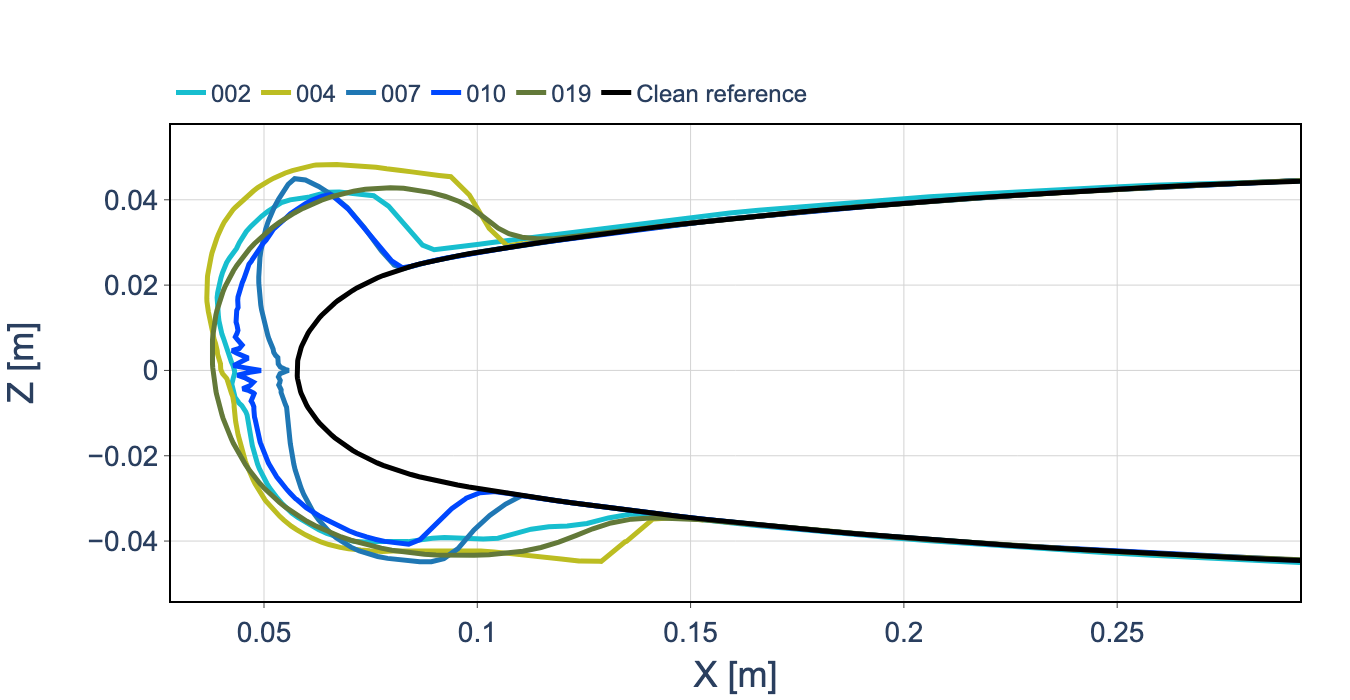
\includegraphics[width=\textwidth]{FIGURES/ICE_SHAPES/tc_oneram6_L1_single_layer_ice_shape_slice_0p1_bins15_roughness_1mm.png}

    \vspace{0.05cm}

    {\scriptsize\textbf{$y=0.10$ m}}
\end{column}

\begin{column}{0.50\textwidth}
    \centering

    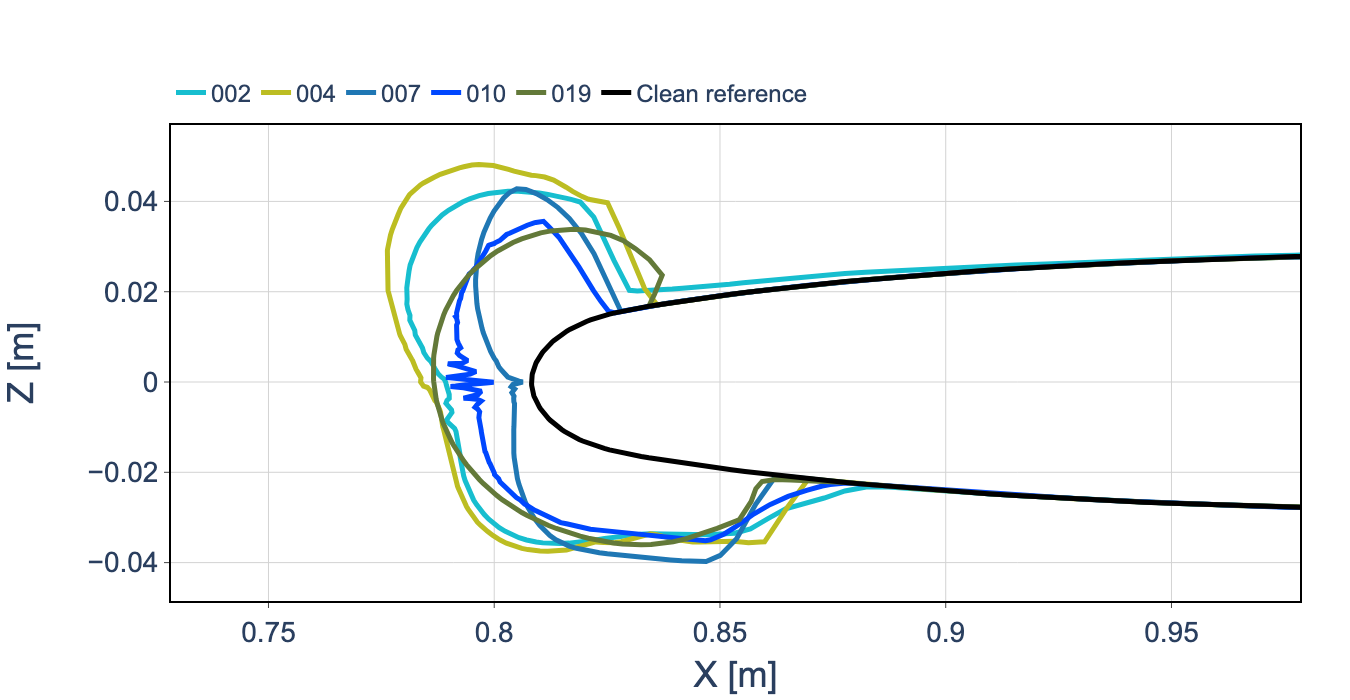
\includegraphics[width=\textwidth]{FIGURES/ICE_SHAPES/tc_oneram6_L1_single_layer_ice_shape_slice_1p4_bins15_roughness_1mm.png}

    \vspace{0.05cm}

    {\scriptsize\textbf{$y=1.40$ m}}
\end{column}

\end{columns}

}

\vspace{0.15cm}

\begin{block}{\scriptsize Assessment}
\begin{itemize}
    \item Considerable code-to-code variability is observed in the predicted ice shape, particularly in horn height, orientation, and local accretion thickness.
    \item Despite these differences, the submissions predict a broadly similar overall accretion region around the leading edge.
    \item<2-> Similar code-to-code variability is observed at the other spanwise locations.
    \item<2-> The geometric spread is consistent with the differences previously observed in the thermodynamic predictions, despite comparatively good agreement in water impingement.
\end{itemize}
\end{block}

\end{frame}

% ============================================================
% ONERA M6 -- Multilayer Ice Shapes
% ============================================================

\begin{frame}{\small ONERA M6 -- Multilayer Ice-Shape Comparison}
\scriptsize

% ------------------------------------------------------------
% Middle slice
% ------------------------------------------------------------
\only<1>{
\centering
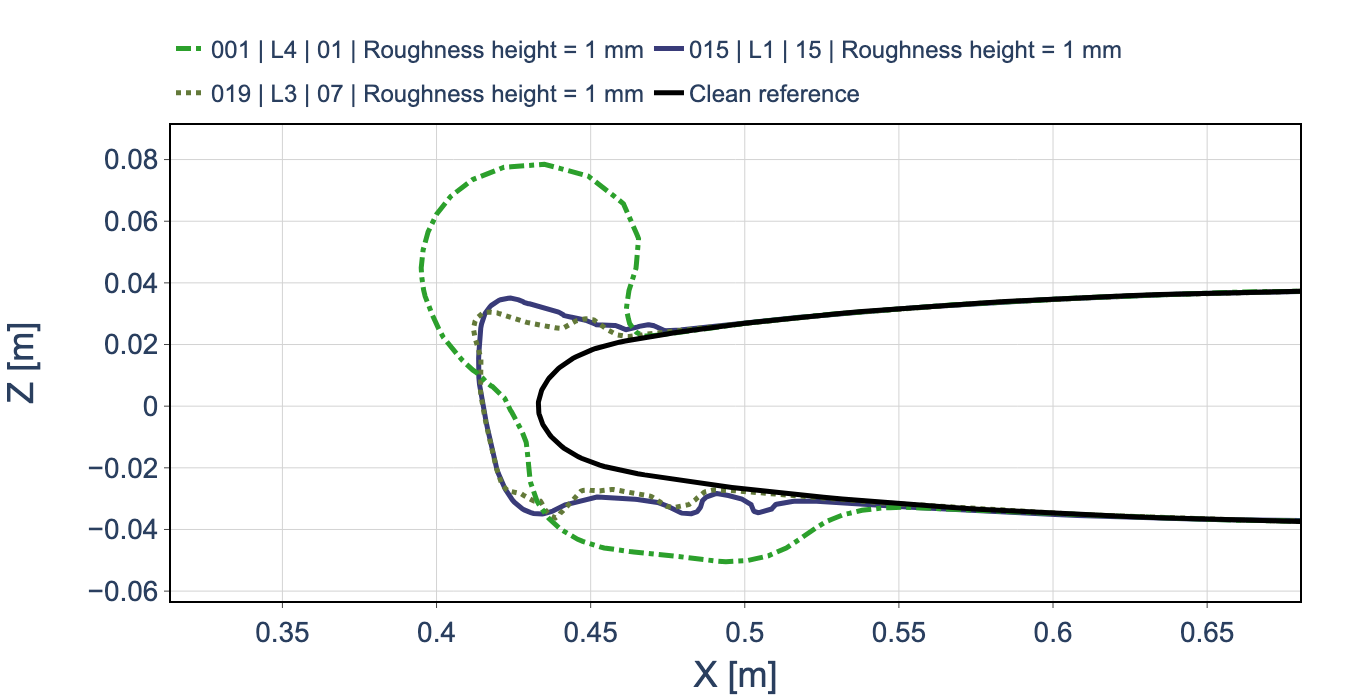
\includegraphics[width=0.70\textwidth]{FIGURES/ICE_SHAPES/tc_oneram6_finest_grid_multilayer_ice_shape_slice_0p75_all_conditions.png}

\vspace{0.05cm}

\textbf{$y=0.75$ m}
}

% ------------------------------------------------------------
% Inboard and outboard slices
% ------------------------------------------------------------
\only<2>{
\begin{columns}[T,onlytextwidth]

\begin{column}{0.50\textwidth}
    \centering
    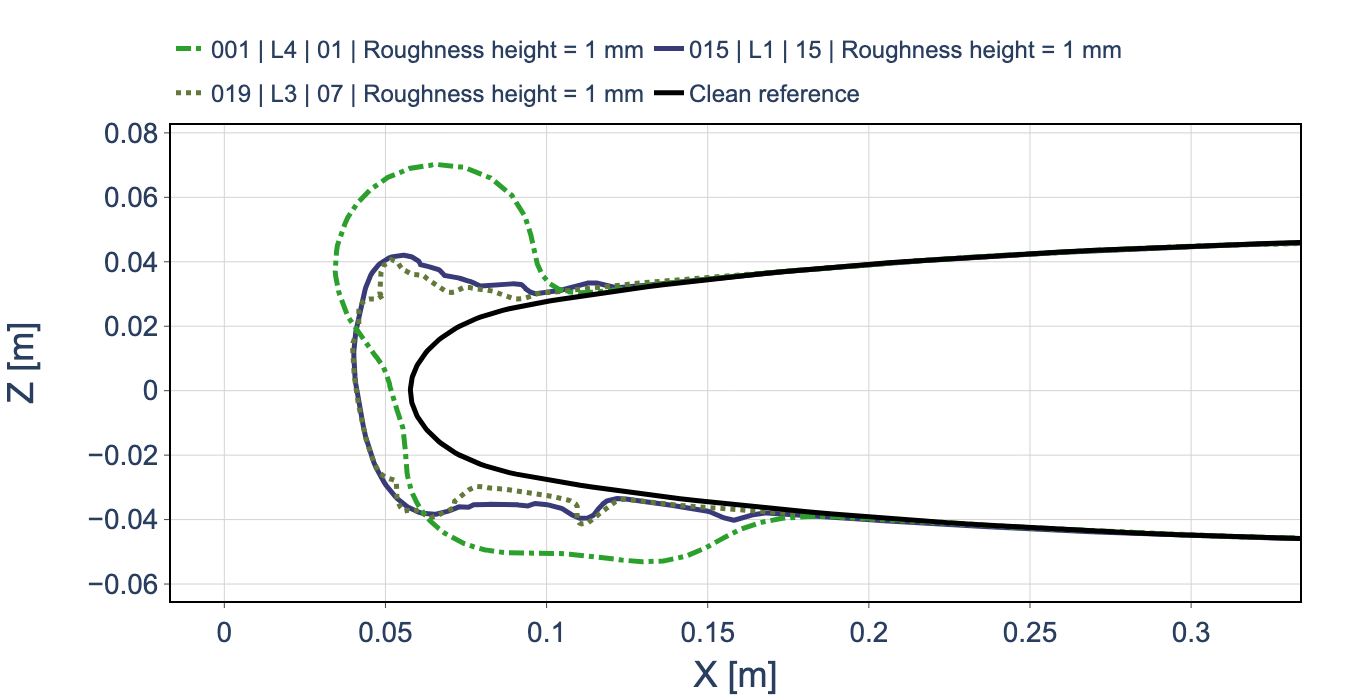
\includegraphics[width=0.94\textwidth]{FIGURES/ICE_SHAPES/tc_oneram6_finest_grid_multilayer_ice_shape_slice_0p1_all_conditions.png}

    \vspace{0.05cm}

    \textbf{$y=0.10$ m}
\end{column}

\begin{column}{0.50\textwidth}
    \centering
    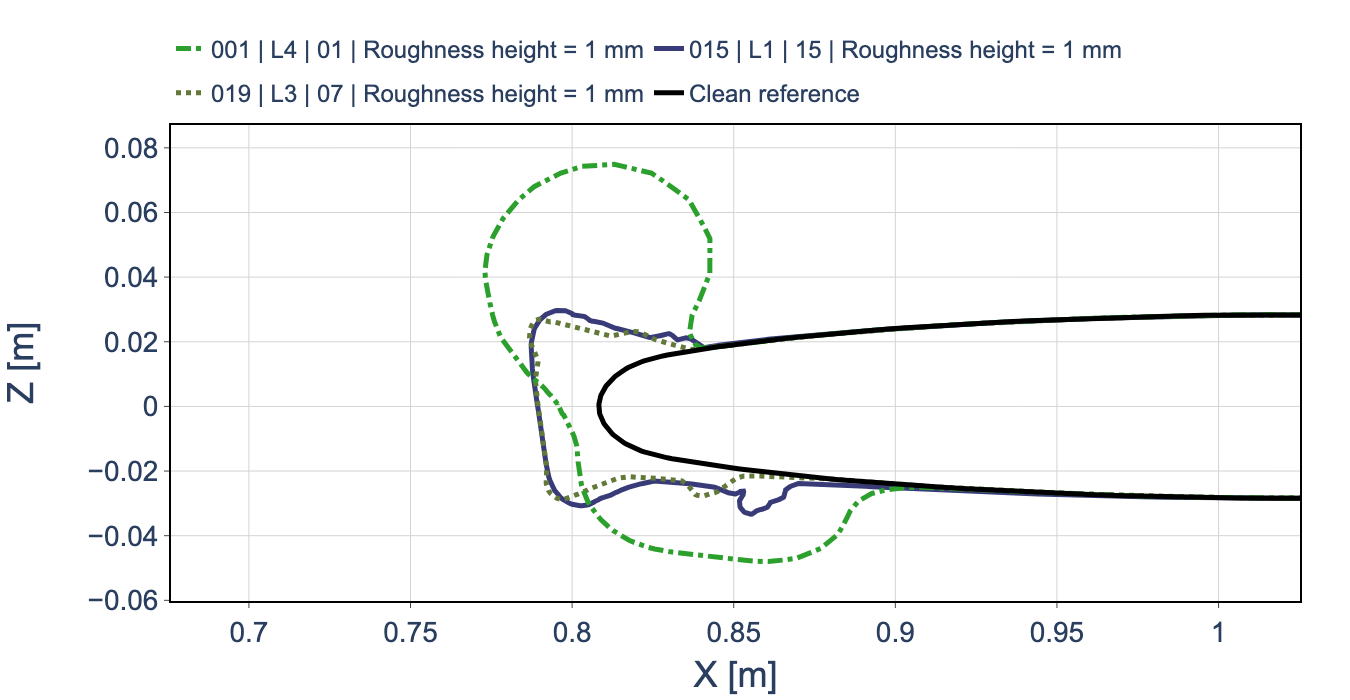
\includegraphics[width=0.94\textwidth]{FIGURES/ICE_SHAPES/tc_oneram6_finest_grid_multilayer_ice_shape_slice_1p4_all_conditions.png}

    \vspace{0.05cm}

    \textbf{$y=1.40$ m}
\end{column}

\end{columns}
}

\vspace{0.10cm}

\begin{block}{\scriptsize Assessment}
\begin{itemize}
    \item<1-> Considerable code-to-code variability is observed in horn orientation, extent, and local ice thickness.
    \item<1-> Predicted accretion ranges from relatively compact shapes to substantially larger upper- and lower-surface horns.
    \item<2-> Similar geometric variability persists at the inboard and outboard spanwise stations.
\end{itemize}
\end{block}

\end{frame}


% ============================================================
% ONERA M6 -- Ice Accretion Summary
% ============================================================

\begin{frame}{\small ONERA M6 -- Ice Accretion Summary}
\scriptsize

\begin{block}{\scriptsize Ice Mass}
\begin{itemize}
    \item Grid sensitivity is submission-dependent, while sensitivity to droplet discretization remains limited.
    \item Code-to-code differences remain substantial and generally exceed the grid and droplet-discretization effects.
\end{itemize}
\end{block}

\vspace{0.08cm}

\begin{block}{\scriptsize Mass Partition}
\begin{itemize}
    \item Most submissions convert approximately $85$--$89\%$ of the impinged water mass into ice.
    \item Evaporation closes much of the remaining mass balance; lower ratios for some submissions are consistent with reported water shedding.
\end{itemize}
\end{block}

\vspace{0.08cm}

\begin{block}{\scriptsize Ice Geometry}
\begin{itemize}
    \item Considerable code-to-code variability is observed in horn height, orientation, and local ice thickness.
    \item Similar geometric variability persists across the three spanwise sections.
\end{itemize}
\end{block}

\vspace{0.08cm}

\begin{alertblock}{\scriptsize Ice Accretion Takeaway}
Good agreement in water impingement does not translate into comparable ice accretion; substantial differences emerge in mass partition and final ice geometry, highlighting the influence of the thermodynamic treatment.
\end{alertblock}

\end{frame}
